\documentclass[11pt]{article}
\usepackage[margin=1in]{geometry}
\usepackage[T1]{fontenc}
\usepackage{amsmath,amssymb,booktabs,graphicx,natbib,hyperref,placeins}
\setlength{\emergencystretch}{2em}
\hypersetup{colorlinks=true,urlcolor=blue,citecolor=blue}
\title{Choosing price forecasts for cryptocurrency sales}
\author{Lai Jien Weng\\Monash University\\\texttt{lai.jienweng@monash.edu}}
\date{}
\begin{document}\maketitle
\begin{abstract}
A forecast can predict the final price well yet guide costly sale timing. We test whether selecting forecasts by trading outcomes improves on selection by final-price error. Seven candidates, including a no-signal baseline, are evaluated using preceding-month data. In 26,496 hypothetical SOL, BNB and XRP sales, execution-based selection improves the model objective relative to final-price selection by 0.0156 basis points, but underperforms the baseline. A simpler rule scoring price differences within the trading period makes identical choices. The evidence supports evaluating forecast paths, while showing that beating a prediction-based selector does not establish profitable execution. Costs are assumed and the test is retrospective.
\end{abstract}
\noindent\textbf{Keywords:} forecast selection; optimal execution; cryptocurrency; transaction costs.\\
\textbf{JEL:} C53; G11; G14.

\section{Introduction}
A trader required to sell a fixed quantity over fifteen minutes must choose how much to sell at each minute. Execution models balance impact and inventory costs \citep{almgren2001} and use predictive signals to adjust trades \citep{cartea2016,lehalle2019,neuman2022,bank2026}. A final-price forecast leaves prices within that period unspecified. Errors about price differences across sale times may therefore matter more than errors about the final price.

Decision-focused learning evaluates predictions through their decision losses \citep{elmachtoub2022,mandi2024}. \citet{kweon2024} already apply this approach to forecasts of liquidity used in adaptive execution. Economic forecast evaluation also appears in portfolio allocation \citep{maciel2025}. We examine a narrower question: when the forecasting models are already fitted, does the criterion used to select among them change execution outcomes? We compare final-price error, full-path error, demeaned-path error and execution objective using identical candidates and access to the no-signal alternative.

Demeaning removes common price-level errors, which cannot change the timing of a compulsory sale. The comparison therefore tests whether execution-based selection adds information beyond this simple adjustment. In newly analysed historical assets, it improves on final-price selection but makes exactly the same choices as demeaned-path selection. Both lose against the baseline. This separates a benefit relative to a prediction-based selector from evidence that forecast-driven trading is worthwhile.

Actual execution requires liquidity and cost measurements. Stochastic-impact models \citep{fouque2022}, cryptoasset impact estimates \citep{barucci2023} and limit-order studies \citep{schnaubelt2022} address mechanisms absent from our minute-bar replay. Fragmentation also limits transfer from one exchange \citep{makarov2020,almeida2024}. Our comparisons concern the specified execution model.

\section{Methodology}
For sales $u\geq0$ with $\mathbf1^\top u=1$ across $N=15$ slots, define
\[
J_p(u)=K(u)-p^\top u,\qquad
K(u)=\eta N\|u\|^2+\frac rN\|\mathbf1-Lu\|^2,
\]
where $L$ accumulates sales and $p$ measures prices in basis points relative to the decision-time open. The baseline minimizes $K$; a forecast $\mu$ produces $u(\mu)=\arg\min J_\mu(u)$. Primary costs are $\eta=2$, $r=1$; all six combinations of $\eta\in\{0.5,2,5\}$ and $r\in\{0,1\}$ are retained. The inventory penalty is a preference, and costs are assumed.

For feasible equality-constrained solutions, let $H=\nabla^2K$, $z=H^{-1}\mathbf1$ and $Q=H^{-1}-zz^\top/(\mathbf1^\top z)$. Baseline-relative gain satisfies
\[
G(\mu,p)=\tfrac12p^\top Qp-\tfrac12(\mu-p)^\top Q(\mu-p).
\]
Thus maximizing calibration gain minimizes a weighted forecast error. When $r=0$, $Q=(I-\mathbf1\mathbf1^\top/N)/(2\eta N)$: execution-based selection equals demeaned-path-error selection if the equality solutions are nonnegative. Binding constraints can break this expression. This standard quadratic identity explains the control; it is not a new execution theory \citep{forde2022,abijaber2025}. Appendix B gives the proof and constraint audit.

Binance spot minute bars cover 1 January 2026 00:00 through 31 August 2026 23:59 UTC \citep{binance2026}. The primary transfer assets are SOLUSDT, BNBUSDT and XRPUSDT. Previously inspected BTCUSDT and ETHUSDT are reported separately. Training/calibration/evaluation months roll from January/February/March through June/July/August. Decisions occur at 00:05, 00:35 through 23:35 daily. Features use completed bars and the decision-time open; execution proxies use opens one to fifteen minutes later. The transfer sample contains 26,496 episodes across 184 dates.

Every selector chooses among seven candidates: zero, the training mean path, three intercept-plus-predictor OLS models, and two ridge models. The OLS predictors are one-minute imbalance, five-minute imbalance and five-minute return. Ridge combines one- and five-minute imbalance and returns with log five-minute volume, using training-only standardization and fixed penalties 0.1 and 1.0. Appendix A specifies the features and fitting objective.

Calibration selects the lowest final-price MSE, full-path MSE or demeaned-path MSE, or the highest mean execution gain. Demeaning subtracts each path's own mean across fifteen prices before scoring its error. Every rule includes zero and uses the same tie order, favouring zero first. One model is then held fixed for the next evaluation month. No rule receives extra shrinkage choices.

We froze the design on 20 September 2026 before computing these outcomes. Motivation came from earlier BTC/ETH results, so this is historical asset transfer, not prospective confirmation \citep{arnott2019}. The primary contrast is execution-based minus final-price selection at $\eta=2,r=1$. Conditional intervals use 4,000 circular moving-block draws of seven consecutive dates, retaining assets together and fitted decisions fixed. One- and fourteen-day blocks are sensitivity checks. Block resampling addresses local dependence \citep{politis1994}, but cannot guarantee validity under arbitrary dependence or propagate full retraining uncertainty. Secondary intervals are unadjusted for multiple comparisons.

\section{Results and discussion}
Execution-based selection improves the model objective relative to final-price selection by 0.01564 basis points, with conditional 95\% interval $[0.00278,0.03184]$. All four selectors nevertheless lose against the no-signal schedule (Table~\ref{tab:selection}). The execution-based rule chooses zero in eleven of eighteen transfer asset-month cells. Each of its seven nonzero choices subsequently loses against that baseline. Access to abstention alone therefore does not eliminate selection error.

\begin{table}[htbp]\centering\small
\caption{Primary transfer outcomes relative to the no-signal schedule, in basis points. Intervals condition on fitted forecasts and selections.}
\label{tab:selection}
\resizebox{\linewidth}{!}{\begin{tabular}{lrrr}
\toprule
Selector & Mean gain & Conditional 95\% interval & Zero choices \\
\midrule
Endpoint MSE & -0.02043 & [-0.03701, -0.00740] & 8/18 \\
Path MSE & -0.01604 & [-0.03171, -0.00416] & 9/18 \\
Contrast MSE & -0.00479 & [-0.00766, -0.00221] & 11/18 \\
Economic & -0.00479 & [-0.00766, -0.00221] & 11/18 \\
Zero baseline & 0.00000 & [0.00000, 0.00000] & 18/18 \\
\bottomrule
\end{tabular}
}
\end{table}

Demeaned-path and execution-based selection agree in all eighteen transfer cells under every cost scenario. They also agree in all twelve BTC/ETH cells at primary costs. The simpler metric therefore reproduces the observed model choices; this is not evidence of an additional benefit from cost-based weighting. Constraints bind for some candidates, so the empirical agreement extends beyond cases guaranteed by the interior formula. Superiority over ordinary full-path MSE remains unresolved: the paired mean difference is 0.01125 basis points, with interval $[-0.00006,0.02664]$.

The primary endpoint comparison remains positive across all six cost scenarios and the three block lengths. However, SOL supplies about 81\% of the pooled improvement and March about 79\% (Figure~\ref{fig:months}). Omitting March leaves a positive descriptive mean of 0.00397 basis points, without refitting. On previously inspected BTC/ETH, the difference is $-0.00077$, with interval $[-0.00670,0.00331]$. Thus the transfer result does not establish uniform superiority across assets.

\begin{figure}[htbp]\centering
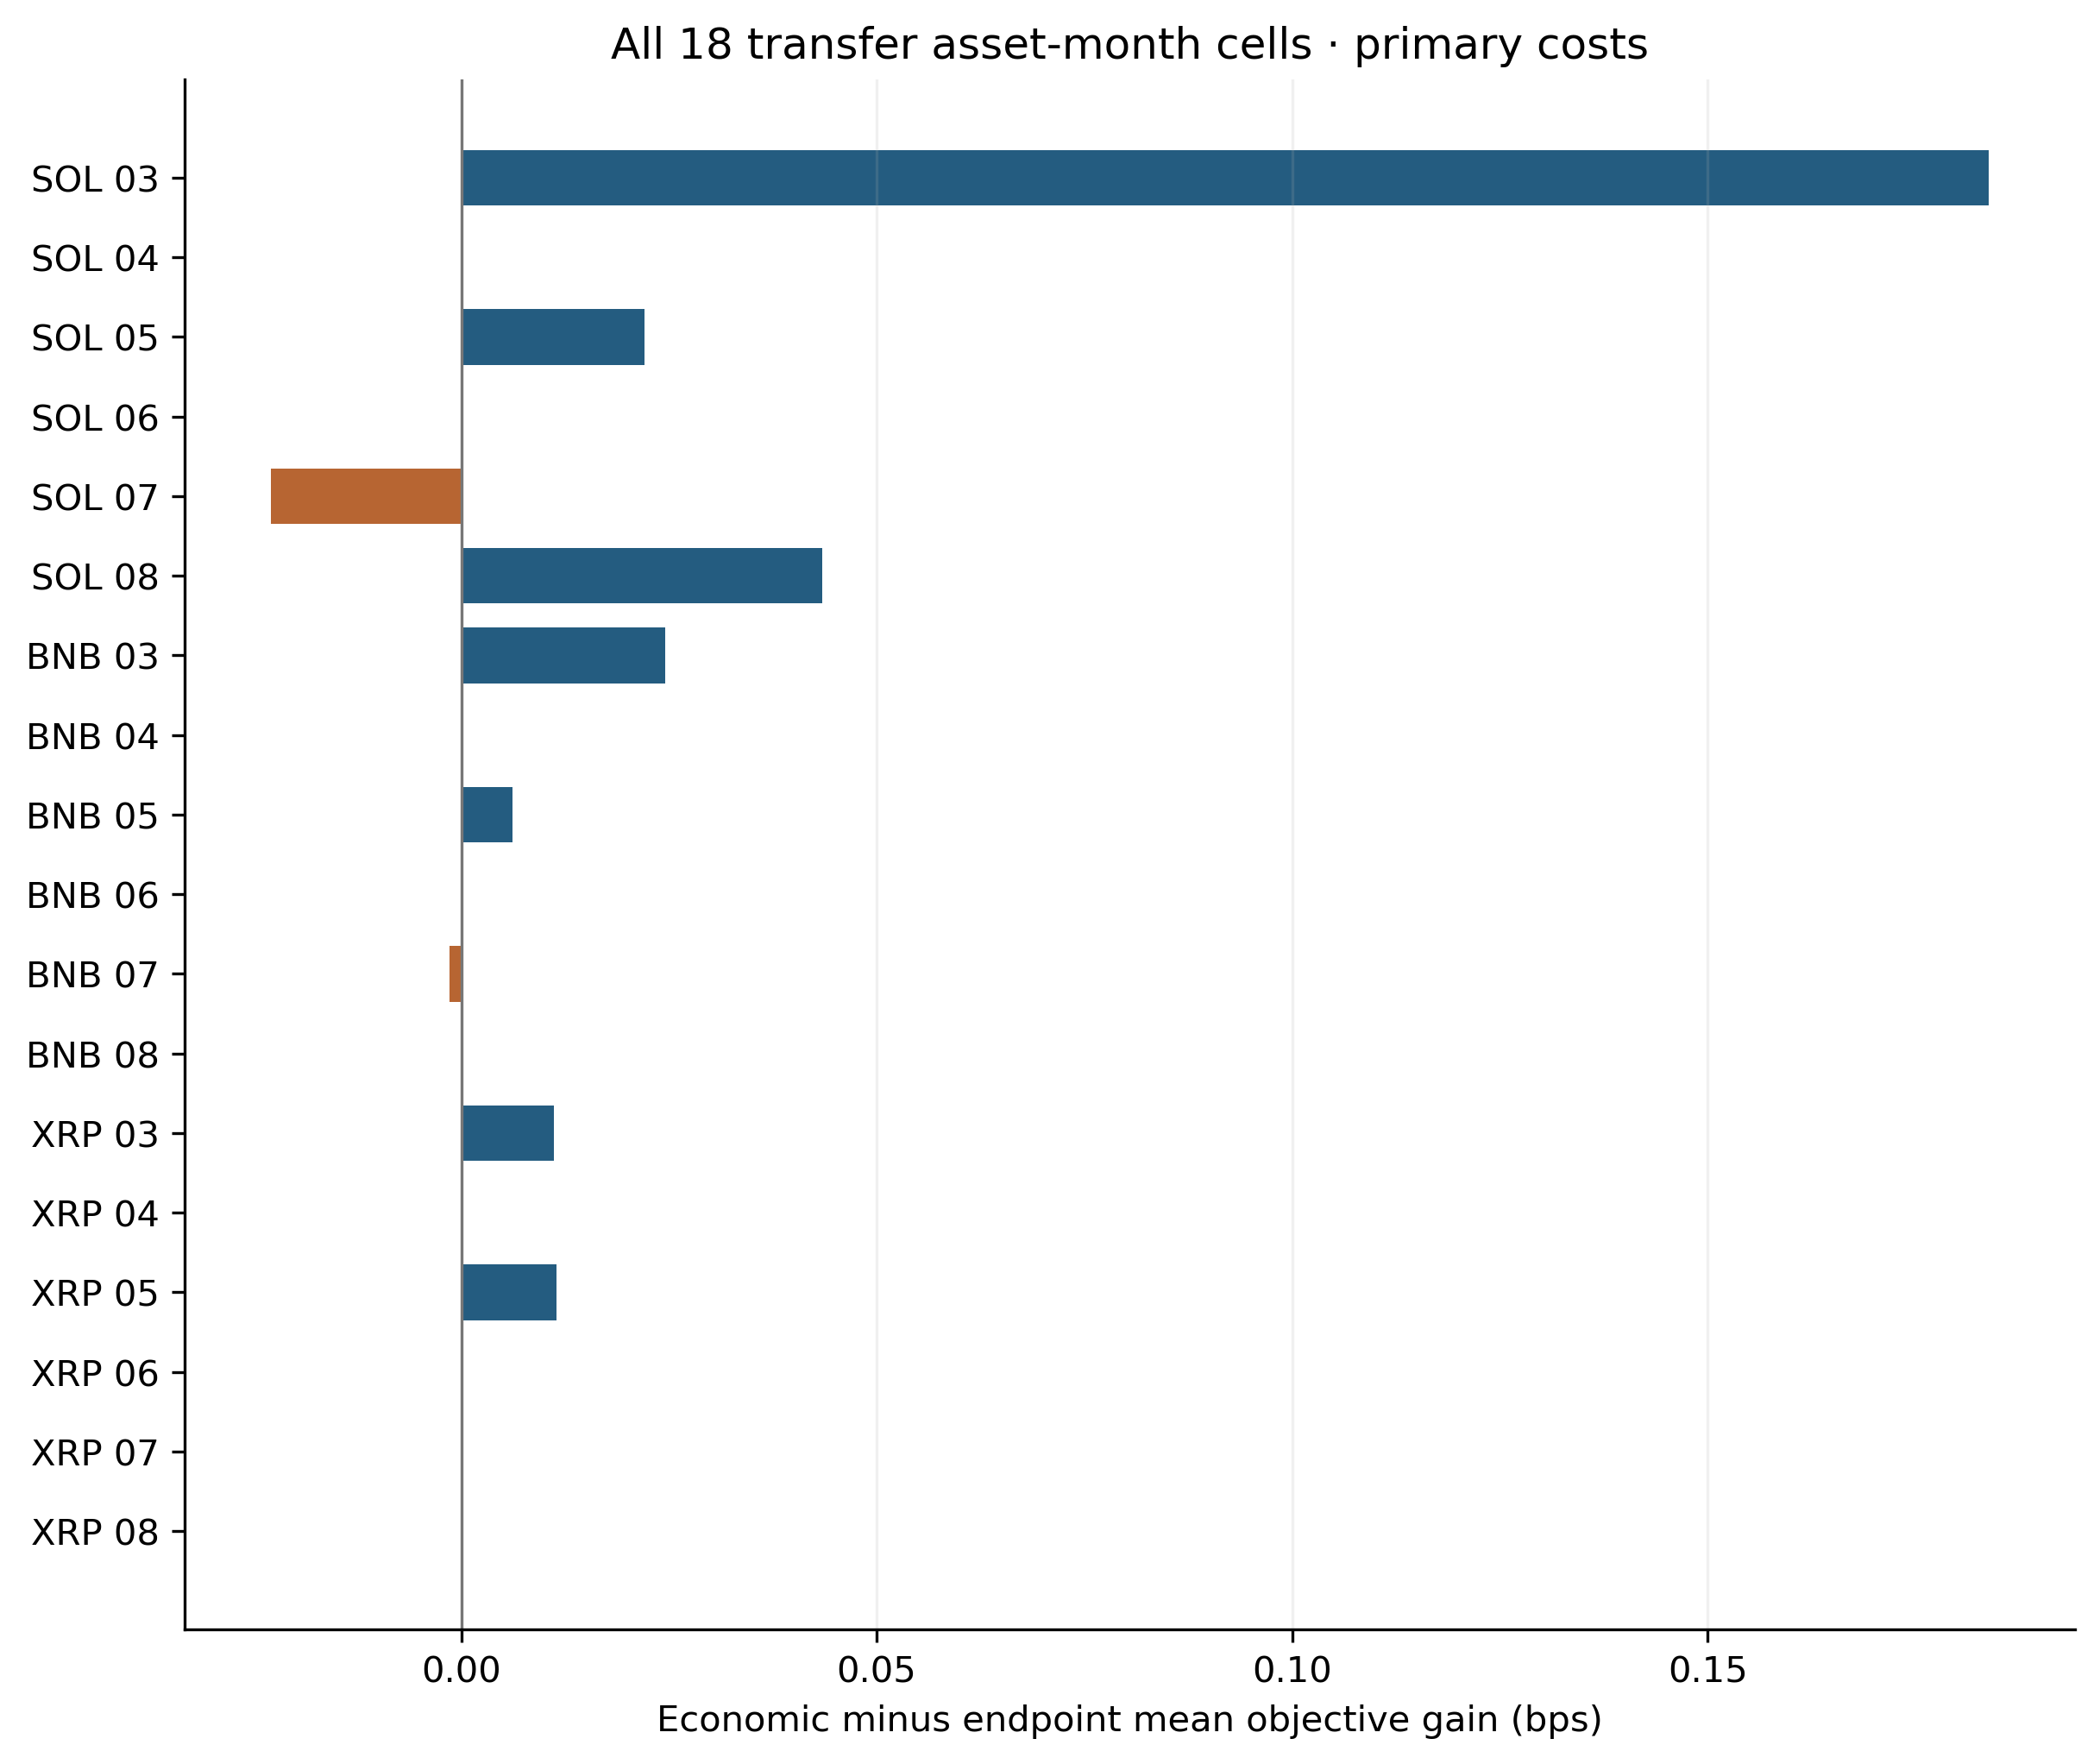
\includegraphics[width=\linewidth]{figures/transfer_monthly_differences.png}
\caption{Execution-based minus final-price selection by asset and evaluation month. Values are paired mean objective differences in basis points; the plot includes every transfer cell.}
\label{fig:months}
\end{figure}

The primary improvement is 1.56 parts per million of reference notional. With $r=0$ and $\eta=2$, the monetary-objective comparison is positive at 0.01592 basis points, but still uses assumed impact. These small differences cannot be interpreted as attainable savings without observed spreads, depth, fills and order sizes. The evidence concerns which errors a selector penalizes: final-price scoring can prefer a different model from scoring price differences across sale times, while the no-signal alternative remains essential.
\FloatBarrier
\section{Conclusion}
Selecting forecasts by their previous-month execution objective produces lower modelled losses than final-price selection in the SOL/BNB/XRP test. Demeaned-path error makes the same choices, providing a simpler account of the observed difference. Neither rule beats the no-signal schedule, and the BTC/ETH comparison is inconclusive. A useful evaluation must therefore compare both forecast-selection criteria and the decision to change the baseline at all. Prospective tests with measured execution costs are needed to establish whether the within-path criterion improves real trading decisions.

\section*{Declarations and availability}
No funding was received; the author declares no competing interests. OpenAI Codex assisted research, coding, analysis, drafting and internal review; the author remains responsible. Public aggregate data and hypothetical orders are used. The frozen protocol, code and results accompany this draft; the existing repository is \url{https://github.com/JienWeng/crypto-execution-timing}.
\begingroup\raggedright\bibliographystyle{plainnat}\bibliography{references}\endgroup
\end{document}
